\documentclass[11pt,a4paper]{article}

% -------- Packages --------------------------------------
\usepackage[utf8]{inputenc}
\usepackage[T1]{fontenc}
\usepackage{lmodern}
\usepackage{graphicx}
\usepackage{xcolor}
\usepackage{tikz}
\usetikzlibrary{shapes.geometric, arrows.meta, positioning, fit, calc, backgrounds}
\usepackage{hyperref}
\usepackage{enumitem}
\usepackage{tcolorbox}
\usepackage{fancyhdr}
\usepackage{geometry}
\geometry{margin=2.5cm}
\setlength{\parskip}{0.7em}
\setlength{\parindent}{0pt}
\setlength{\headheight}{13.6pt}
\addtolength{\topmargin}{-1.6pt}

% -------- Header / Footer --------------------------------
\pagestyle{fancy}
\fancyhf{}
\fancyhead[L]{\textbf{Apeiron Explained}}
\fancyhead[R]{\thepage}
\renewcommand{\headrulewidth}{0.4pt}

% -------- Title ------------------------------------------
\title{\textbf{The Apeiron Framework}\\[0.3em]
\Large A gentle introduction to an AI that builds its own knowledge from scratch}
\author{David Beniers}
\date{\today}

\begin{document}
\maketitle
\thispagestyle{empty}
\vspace*{\fill}
\newpage

% -------- Teaser -----------------------------------------
\section*{Imagine This...}
\addcontentsline{toc}{section}{Imagine This...}

\begin{tcolorbox}[colback=black!3, colframe=black!40, title=\textbf{A Message from the Author}]
A robot wakes up on the red dust of Mars.  Its name is \textbf{Pixel}.
The rover that carried it has crashed; its communication antenna is
shattered.  Pixel has one working camera, no map, and no instructions.
It must learn to see, to think, to plan – entirely on its own – if it
wants to signal Earth and save the mission.

This is the dream behind \textbf{Apeiron}.
\end{tcolorbox}

% -------- Sections ---------------------------------------
\section*{About This Document}
\addcontentsline{toc}{section}{About This Document}

This booklet is a friendly, illustrated guide to the \textbf{Apeiron Framework}---a
research programme that tries to build an artificial intelligence that can
create its own knowledge \emph{from scratch}, without using any human labels,
categories, or pre‑defined goals.

You do not need to know mathematics, programming, or philosophy beforehand.
Every new idea is explained step by step, with plenty of pictures and a
continuous story that follows a little robot called \textbf{Pixel}.

By the time you reach the last page, you will understand:
\begin{itemize}
    \item why today’s AI is not as smart as it seems,
    \item how a machine could observe the world without any human help,
    \item what the seventeen layers of Apeiron do, and
    \item why this matters for the future of intelligent machines.
\end{itemize}

Let’s begin!

\vspace{1em}
\textit{“I started building Apeiron because I believe that the most
interesting things in the universe are the ones we do not yet have a name
for.  This framework is my attempt to create a machine that can show us
those things.”} \hfill – David Beniers
\section{What Does It Mean to ``Know'' Something?}
\label{sec:intro}

Imagine you see a chair for the first time.  Nobody tells you what it is,
yet you quickly understand that you can sit on it.  How does your brain
figure that out?

Your brain detects shapes, colours, and edges.  It notices that certain
groups of shapes often appear together, and it learns to associate those
groups with the possibility of sitting.  Over time, you build a mental
model of the world that is independent of any single teacher.

Today’s artificial intelligence systems are \emph{not} like that.  They
are trained on millions of pictures that already have labels attached:
“chair”, “cat”, “car”.  They never have to discover the concept of a
chair by themselves.

The Apeiron Framework asks a bold question:
\begin{center}
\textbf{What if an AI had to build \emph{all} its knowledge from
elementary observations, without ever being told what anything means?}
\end{center}

\subsection*{A Small Glimpse of What Apeiron Already Does}

Look at the two rows of images below.
They are photographs of the real world, but they have no captions.
Apeiron looked at 3000 such photos and found a group of pixels that
fires together – a texture pattern, a contrast between light and dark –
that appears in aeroplanes, deer, ships, and frogs alike.
No human labelled this pattern; it is simply a signal that the world
offers, and Apeiron picked it up.

\begin{figure}[ht]
  \centering
  
\includegraphics[width=0.9\textwidth]{figures/cifar_cluster_example.pdf}
  \caption{Left block: images where the most active Apeiron feature cluster
           is prominent. Right block: images where it is scarcely present.
           The cluster captures high‑contrast textures that recur across
           object classes.}
  \label{fig:cifar_example}
\end{figure}

\subsection*{Meet Pixel – Our Little Explorer}

To make all of this concrete, we will follow a tiny robot called \textbf{Pixel}.
Pixel has crash‑landed on Mars next to a broken rover.  Its only working
sensor is a camera, and its only goal is to understand the world well
enough to repair the antenna and call Earth.  Step by step, we will
watch Pixel climb the same seventeen‑layer ladder that Apeiron uses,
from raw sensation to a full‑blown plan of action.

So, grab a comfy seat and let’s join Pixel on its journey!
\section{The Limits of Today’s AI}
\label{sec:limits}

Modern AI can recognise faces, translate languages, and even drive cars.
But under the hood, these systems are \emph{statistical mirrors}: they
reflect the patterns that humans have already put into the data.

\begin{tcolorbox}[colback=blue!5, colframe=blue!40, title=Quick thought]
If you train an AI on 10\,000 labelled photos of cats and dogs, it
becomes very good at telling cats from dogs.  Yet it has no idea what
a cat \emph{is} – it only knows that a certain pixel pattern usually
comes with the label “cat”.
\end{tcolorbox}

Three problems arise from this approach:
\begin{enumerate}
    \item \textbf{Every concept must be predefined.}  The AI cannot invent
    a new category that a human did not already think of.
    \item \textbf{Time is treated as a fixed step.}  The AI does not
    experience the world as a flow of events.
    \item \textbf{Bias is baked in.}  If the training data contains
    stereotypes, the AI will reproduce them.
\end{enumerate}

\begin{tcolorbox}[colback=red!5, colframe=red!40, title=The Parrot and the Scientist]
Think of today’s large language models as a \textbf{parrot}.  The parrot
hears the word “water” thousands of times and learns to say it in the
right context.  But it has never touched water, never tasted it, never
felt its weight.  It has no idea what water really \emph{is}.

Now imagine a \textbf{scientist} who has never heard the word “water”.
She studies a puddle: she measures its temperature, watches how it
evaporates, sees how it reflects light.  She builds a concept —
“that transparent, flowing thing that disappears in sunlight” — and
gives it her own name.  Her understanding is grounded in observation,
not in borrowed vocabulary.

Apeiron is the scientist.  It does not repeat what humans have said;
it builds knowledge from the ground up.
\end{tcolorbox}

\begin{tcolorbox}[colback=red!5, colframe=red!40, title=Why Apeiron is fundamentally different]
Apeiron does \emph{not} try to make a better version of today’s AI.
It is a completely different path — one that starts with raw sensory
data and lets structure emerge on its own, without any human‑provided
labels, categories, or clocks.  Think of it not as a faster car, but
as the first spaceship.
\end{tcolorbox}
\section{The Core Idea of Apeiron}
\label{sec:idea}

The name “Apeiron” comes from an ancient Greek word meaning
\emph{the unlimited} or \emph{the source of all things}.  The framework
is built on a simple philosophy:
\begin{quote}
\textbf{Intelligence is the ability to organise elementary observations
into coherent, useful knowledge without any external guidance.}
\end{quote}

\begin{tcolorbox}[colback=purple!5, colframe=purple!50, title=\textbf{Where does the name come from?}]
More than 2500 years ago, the Greek thinker Anaximander proposed that
everything in the universe arose from a single, boundless substance he
called \emph{to apeiron} — “the unlimited”.  It was not water, not
fire, but something deeper from which all things emerge and to which
they return.

The Apeiron Framework borrows this idea: intelligence, too, can emerge
from a single, undivided starting point — raw observation — and
gradually unfold into a rich universe of concepts.  No pre‑defined
categories, no imported labels; just an open field of possibilities,
waiting to be structured.
\end{tcolorbox}

\begin{figure}[ht]
\centering
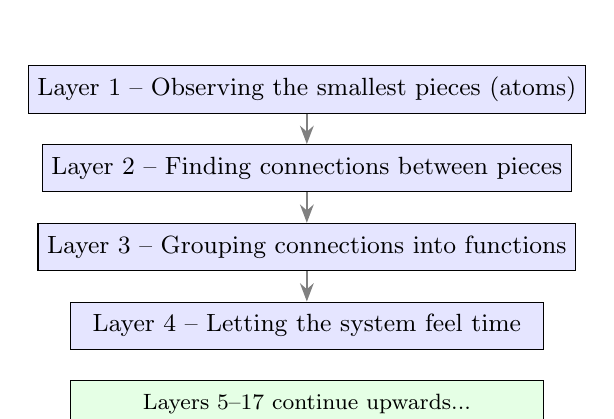
\begin{tikzpicture}[
    layer/.style={rectangle, draw=black, fill=blue!10, minimum width=6cm, minimum height=0.6cm, font=\small},
    arrow/.style={-{Stealth}, thick, gray}
]
\node[layer] (L1) at (0,0)  {Layer 1 – Observing the smallest pieces (atoms)};
\node[layer] (L2) at (0,-1) {Layer 2 – Finding connections between pieces};
\node[layer] (L3) at (0,-2) {Layer 3 – Grouping connections into functions};
\node[layer] (L4) at (0,-3) {Layer 4 – Letting the system feel time};
\node[layer, fill=green!10] at (0,-4) {\footnotesize Layers 5–17 continue upwards...};
\foreach \i in {1,2,3} {
    \pgfmathtruncatemacro{\j}{\i+1}
    \draw[arrow] (L\i.south) -- (L\j.north);
}
\end{tikzpicture}
\caption{The first four layers of Apeiron (simplified).  Each layer builds upon the one below it.}
\label{fig:layers_simple}
\end{figure}

Apeiron has \textbf{seventeen layers} organised in four clusters.
But don’t worry – we will look at every single one, step by step,
following Pixel’s journey on Mars.
\section{Layer~1 – The Atoms of Observation}
\label{sec:layer1}

% ----- SUPERKRACHT -----
\begin{tcolorbox}[colback=blue!5, colframe=blue!60, title=\textbf{Superpower: The Splitter}]
\begin{center}
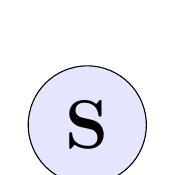
\begin{tikzpicture}
  \node[draw, circle, fill=blue!10, minimum size=1.5cm, font=\bfseries\Huge] {S};
\end{tikzpicture}
\textit{“Is this indivisible?”}
\end{center}
\end{tcolorbox}

Every building needs raw materials.  For Apeiron, the raw material is
something called an \textbf{Ultimate Observable} – a tiny, indivisible
piece of information.  You can think of it as the \emph{quantum} of
experience: the smallest chunk that still carries meaning.

\begin{tcolorbox}[colback=yellow!5, colframe=yellow!80, title=Real‑life analogy]
A 1000‑piece jigsaw puzzle.  You tip the box and a thousand little
cardboard shapes pour out.  Each piece is meaningless by itself, but
together they can become anything.  Apeiron’s Layer~1 is like
carefully picking up one piece, examining it from all sides, and
confirming: \emph{this piece cannot be split further without breaking
the picture it might become.}
\end{tcolorbox}

\textbf{Pixel’s point of view.}
Pixel wakes up and switches on its camera.  It sees a mosaic of tiny
coloured squares – red, blue, green, dark, bright.  That is all it has.
Nobody tells Pixel “this is a rock” or “that is a shadow”.  It just
stares at a sea of numbers.

Pixel asks itself: \emph{is this little square truly basic, or could
I split it into even smaller, still useful pieces?}  If the answer is
“no”, the square becomes an atom – a certified building block of
Pixel’s future knowledge.

\subsection*{Why not just use pixels and be done with it?}

That’s a fair question!  In a digital photo a pixel is already the
smallest dot you can get.  So why go through all the trouble of
inspecting it?  Because Apeiron is not designed only for photos – it
could be fed with sound waves, temperature curves, or the pressure of
a robot’s foot on the ground.  In those worlds, the “smallest
meaningful piece” is not obvious at all.  The four inspectors
guarantee that, whatever the sensor, the system always starts from a
rock‑solid foundation.

\begin{figure}[ht]
\centering
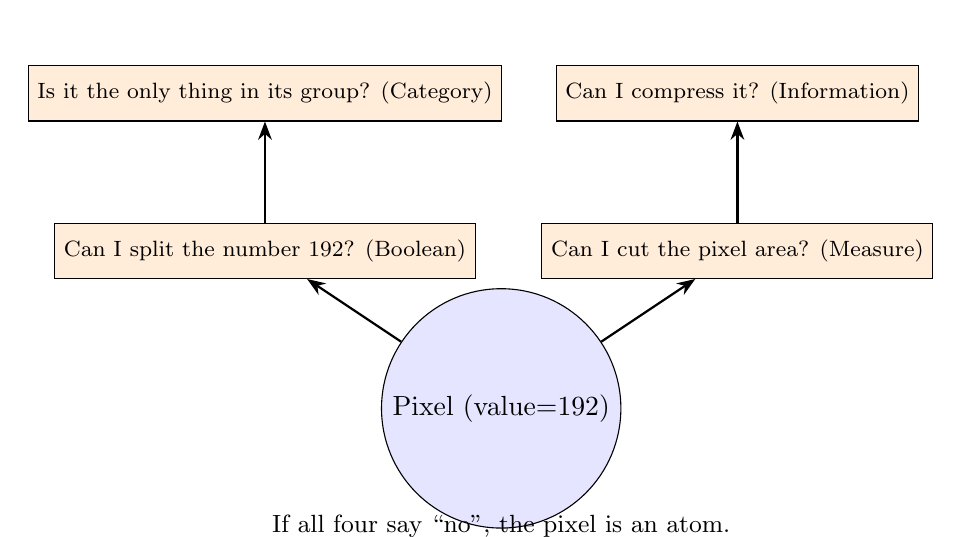
\begin{tikzpicture}[
    checker/.style={rectangle, draw=black, fill=orange!15, minimum width=2.8cm, minimum height=0.7cm, align=center, font=\footnotesize},
    arrow/.style={-{Stealth}, thick}
]
\node (obs) at (0,0) [draw, circle, fill=blue!10] {Pixel (value=192)};
\node (B) at (-3, 2) [checker] {Can I split the number 192? (Boolean)};
\node (M) at (3, 2)  [checker] {Can I cut the pixel area? (Measure)};
\node (C) at (-3, 4) [checker] {Is it the only thing in its group? (Category)};
\node (I) at (3, 4)  [checker] {Can I compress it? (Information)};
\draw[arrow] (obs) -- (B);
\draw[arrow] (obs) -- (M);
\draw[arrow] (B) -- (C);
\draw[arrow] (M) -- (I);
\node at (0,-1.5) {\small If all four say “no”, the pixel is an atom.};
\end{tikzpicture}
\caption{The four mathematical inspectors that certify atomicity.}
\label{fig:atomicity}
\end{figure}

\subsection*{A peek into Pixel’s inspector room}

Imagine Pixel sitting at a desk, a magnifying glass in one hand, a
ruler in the other, a philosophy textbook to the left, and a
compression algorithm on its screen.

\begin{itemize}
    \item The \textbf{Boolean Inspector} mutters: “Hmm, 192 is divisible
    by 2, by 3… but only 1 and itself count.  No proper divisors?  Atom!”
    \item The \textbf{Measure Inspector} measures the pixel area: “If I
    cut this in half, each half still behaves like a pixel?  Yes – so
    it’s safe.”
    \item The \textbf{Category Inspector} looks around: “Is this pixel
    the only one of its kind?  If I delete it, does the whole thing
    collapse?  No?  Then it’s an atom.”
    \item The \textbf{Information Inspector} ZIP‑compresses the pixel:
    “I tried to squeeze it.  It won’t get any smaller.  That means it
    already contains as much info as it can.  Atom!”
\end{itemize}

All four agree.  Pixel stamps the pixel as \textbf{atomic} and stores
it safely in its memory.

% ----- WAT ALS...? -----
\begin{tcolorbox}[colback=orange!5, colframe=orange!60, title=\textbf{What if...?}]
What if the very first atom Pixel picks is actually a meaningless
speck of dust on the camera lens?  Could the whole knowledge tower
collapse because of a dirty sensor?
\end{tcolorbox}
\section{Layer~2 – From Isolated Dots to a Web of Relations}
\label{sec:layer2}

% ----- SUPERKRACHT -----
\begin{tcolorbox}[colback=blue!5, colframe=blue!60, title=\textbf{Superpower: The Networker}]
\begin{center}
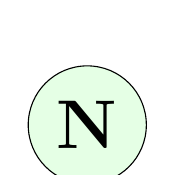
\begin{tikzpicture}
  \node[draw, circle, fill=green!10, minimum size=1.5cm, font=\bfseries\Huge] {N};
\end{tikzpicture}
\textit{“Who talks to whom?”}
\end{center}
\end{tcolorbox}

One atom alone is useless.  It’s like a single word spoken in an empty
room – it has no context, no connection.  Meaning only emerges when
atoms start talking to each other.

\begin{tcolorbox}[colback=yellow!5, colframe=yellow!80, title=Real‑life analogy]
Look at the night sky.  Every star is a lonely point of light.  But
your brain connects them with imaginary lines and sees a bear, a
hunter, a swan.  Those constellations do not exist “out there”; they
exist in the relationships \emph{between} the stars.

Pixel does exactly this with pixels.  A single bright pixel is a star;
when many bright pixels appear close together, Pixel draws a web of
connections between them.  Over time, this web becomes a map of the
world — a \textbf{hypergraph} — that tells Pixel which stars belong to
the same constellation.
\end{tcolorbox}

\textbf{Pixel’s journey continues.}
After many snapshots of the Martian landscape, Pixel notices something:
bright pixels near the horizon often fire together with dark pixels
right next to them.  A strong connection appears.  Other pixel‑pairs
barely ever co‑activate – a weak connection.  Pixel begins to draw a
giant map where every dot is linked to others with a number that says
how tightly they belong together.

\begin{figure}[ht]
\centering
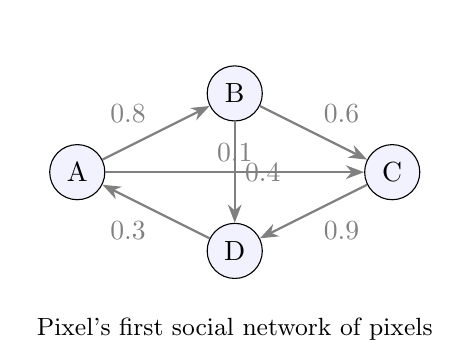
\begin{tikzpicture}[
    node/.style={circle, draw=black, fill=blue!5, minimum size=0.7cm},
    edge/.style={-{Stealth}, thick, color=gray}
]
\node[node] (a) at (0,0) {A};
\node[node] (b) at (2,1) {B};
\node[node] (c) at (4,0) {C};
\node[node] (d) at (2,-1){D};
\draw[edge] (a) -- node[above left] {0.8} (b);
\draw[edge] (b) -- node[above right]{0.6} (c);
\draw[edge] (c) -- node[below right]{0.9} (d);
\draw[edge] (d) -- node[below left] {0.3} (a);
\draw[edge] (a) -- node[above] {0.1} (c);
\draw[edge] (b) -- node[right] {0.4} (d);
\node at (2,-2) {\small Pixel’s first social network of pixels};
\end{tikzpicture}
\caption{Four observables linked by weighted connections.}
\label{fig:network}
\end{figure}

This map is called a \textbf{hypergraph} – a web of relationships that
will later tell Pixel where to look for interesting structures.  Notice
that Pixel still does not know what a “rock” is; it only senses who
co‑occurs with whom.  That is the first, crucial break away from
human‑centered thinking.

\subsection*{Why a hypergraph and not just a simple network?}

In an ordinary social network, you can only be friends with
individuals.  But in the real world, a group of three stars might form
a triangle that has a special meaning.  A hypergraph allows Pixel to
record not only “A talks to B”, but also “A, B, and C light up
simultaneously”.  This ability to see groups, not just pairs, is what
makes the hypergraph such a powerful discovery tool.

\begin{tcolorbox}[colback=blue!5, colframe=blue!40, title=Try this at home]
Open a photo on your phone and zoom all the way in.
Do you see how a patch of sky is made of thousands of tiny squares
that all have very similar colours?  Those squares are strongly
connected in Pixel’s hypergraph — they are his “Milky Way”.
\end{tcolorbox}

% ----- WAT ALS...? -----
\begin{tcolorbox}[colback=orange!5, colframe=orange!60, title=\textbf{What if...?}]
What if Pixel only had one picture to learn from?  Could it still
discover meaningful constellations, or would it be like trying to draw
a map of the sky after seeing only one star?
\end{tcolorbox}
\section{Layer~3 – From Connections to Meaningful Groups}
\label{sec:layer3}

% ----- SUPERKRACHT -----
\begin{tcolorbox}[colback=blue!5, colframe=blue!60, title=\textbf{Superpower: The Grouper}]
\begin{center}
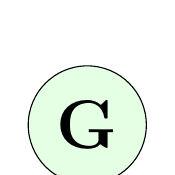
\begin{tikzpicture}
  \node[draw, circle, fill=green!10, minimum size=1.5cm, font=\bfseries\Huge] {G};
\end{tikzpicture}
\textit{“Which pieces belong together?”}
\end{center}
\end{tcolorbox}

Once the social network is drawn, you naturally notice groups: the
sports club, the music band, the chess team.  In the same way, Pixel
now looks for \emph{clusters} – groups of pixels that are so tightly
interlinked that they form a single, functional unit.

\begin{tcolorbox}[colback=yellow!5, colframe=yellow!80, title=Real‑life analogy]
A football team.  Eleven players move in patterns that are much more
coordinated among themselves than with the audience.  If you remove the
goalkeeper, the whole team’s performance drops dramatically.  Apeiron
uses this same logic to decide whether a cluster is important: it
temporarily deletes the cluster and checks if the system becomes
“blind” without it.
\end{tcolorbox}

\textbf{Pixel discovers shapes.}
Pixel finds a tight cluster of pixels in its web.  When it removes that
cluster, it can no longer tell the difference between a picture of the
rover and a picture of empty desert.  The cluster must be doing
something useful!  Without ever hearing the word “wheel” or “antenna”,
Pixel has discovered a \textbf{functional unit}: a reusable pattern
that helps it organise its visual world.

\begin{figure}[ht]
\centering
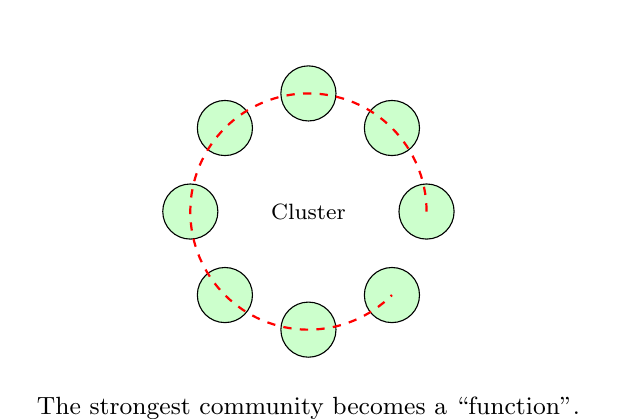
\begin{tikzpicture}[
    c/.style={circle, draw=black, fill=green!20, minimum size=0.7cm}
]
\foreach \i in {0,...,7} {
    \node[c] at (360/8*\i:1.5) {};
}
\node at (0,0) {\footnotesize Cluster};
\draw[red, thick, dashed] (360/8*0:1.5) arc (0:315:1.5);
\node at (0,-2.5) {\small The strongest community becomes a “function”.};
\end{tikzpicture}
\caption{Community detection: tight groups emerge from the network.}
\label{fig:clusters}
\end{figure}

This is a profound moment: Pixel begins to \emph{name} things – not
with human words, but with internal tags that mean “that pattern that
helps me predict what will happen next”.  Knowledge is born.

\subsection*{The ablation test – Pixel’s way of asking “are you important?”}

To check whether a cluster really matters, Pixel performs a
\emph{counterfactual ablation test}: it deletes the cluster from its
memory and tries to do the same tasks as before.  If the performance
drops sharply, the cluster was crucial; if nothing changes, it was
probably just noise.

Imagine you are trying to recognise a friend’s face.  If I erase the
eyes from the photo, you will probably fail.  If I erase a small patch
of cheek, you might not even notice.  That is exactly what Pixel
learns about its own pixel‑groups.

% ----- WAT ALS...? -----
\begin{tcolorbox}[colback=orange!5, colframe=orange!60, title=\textbf{What if...?}]
What if Pixel discovers a cluster that \emph{no human has ever noticed}
– say, a relationship between the angle of the sun and a particular
rock pattern?  Would we be able to understand what it is telling us?
\end{tcolorbox}
\section{Layer~4 – The Birth of Time}
\label{sec:layer4}

% ----- SUPERKRACHT -----
\begin{tcolorbox}[colback=blue!5, colframe=blue!60, title=\textbf{Superpower: The Time Weaver}]
\begin{center}
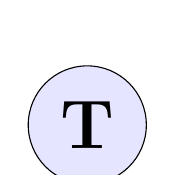
\begin{tikzpicture}
  \node[draw, circle, fill=blue!10, minimum size=1.5cm, font=\bfseries\Huge] {T};
\end{tikzpicture}
\textit{“What happens before what?”}
\end{center}
\end{tcolorbox}

Up to now, Pixel only looked at still pictures.  But the world flows.
A dust storm moves, a shadow creeps across the ground, the rover’s
metal arm bends in the wind.  To understand causality, Pixel needs a
sense of \textbf{time} – not the ticking of a clock, but the order in
which one event leads to another.

\begin{tcolorbox}[colback=yellow!5, colframe=yellow!80, title=Real‑life analogy]
A row of dominoes.  You push the first tile; it falls and pushes the
second; the second pushes the third.  The universe’s own arrow of time
is nothing more than this chain of causes.  Apeiron’s Layer~4 watches
which functional units change \emph{before} others change, and from
those observations it builds its own internal calendar.
\end{tcolorbox}

\textbf{Pixel feels the flow.}
Pixel notices that when a functional unit in the bottom‑left corner
intensifies, a unit in the top‑right corner always brightens half a
second later.  It draws an arrow: \emph{left‑bottom triggers
right‑top}.  Soon Pixel has a dynamic map of the world where past,
present, and future are defined entirely by the causal connections
between its own clusters.

\begin{figure}[ht]
\centering
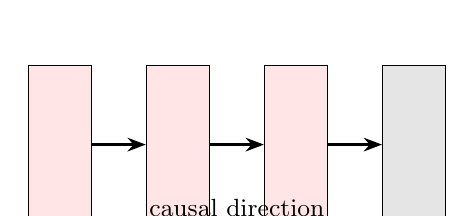
\begin{tikzpicture}[
    dom/.style={rectangle, draw=black, fill=red!10, minimum width=0.8cm, minimum height=2cm},
    arrow/.style={-{Stealth}, thick}
]
\node[dom] (d1) at (0,0) {};
\node[dom] (d2) at (1.5,0) {};
\node[dom] (d3) at (3,0) {};
\node[dom, fill=gray!20] (d4) at (4.5,0) {};
\draw[arrow] (d1) -- (d2);
\draw[arrow] (d2) -- (d3);
\draw[arrow] (d3) -- (d4);
\node at (2.25,-0.8) {\small causal direction};
\end{tikzpicture}
\caption{Apeiron’s “time” is the chain of cause and effect.}
\label{fig:time}
\end{figure}

\subsection*{Why not just use a clock?}

Because the world does not tick!  Some processes are lightning fast
(a flash of lightning), others are painfully slow (the growth of a
tree).  If Pixel used an external clock, it would have to guess the
right speed for everything.  By letting time emerge from the events
themselves, Pixel always moves at exactly the right rhythm for each
situation.

\subsection*{A dash of randomness}

Pixel also adds a tiny bit of noise – deliberate randomness – to its
predictions.  Why?  Because if it always followed the exact same path,
it might get stuck in a rut.  A little exploration lets Pixel discover
new, better ways of organising its world, just like you sometimes try
a new route to school and find a shortcut.

% ----- WAT ALS...? -----
\begin{tcolorbox}[colback=orange!5, colframe=orange!60, title=\textbf{What if...?}]
What if Pixel’s internal clock runs faster than ours?  Could it see
patterns in the Martian dust that happen too slowly for a human to
ever notice?
\end{tcolorbox}

% --- Cluster II ------------------------------------------
\section{Layer~5 – Autonomous Optimization}
\label{sec:layer5}

% ----- SUPERKRACHT -----
\begin{tcolorbox}[colback=blue!5, colframe=blue!60, title=\textbf{Superpower: The Optimiser}]
\begin{center}
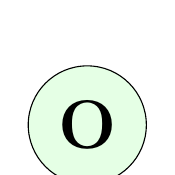
\begin{tikzpicture}
  \node[draw, circle, fill=green!10, minimum size=1.5cm, font=\bfseries\Huge] {O};
\end{tikzpicture}
\textit{“How can I get better at what I do?”}
\end{center}
\end{tcolorbox}

Pixel can now recognise groups of pixels and lay cause‑and‑effect links.
But the world does not stand still, and neither does Pixel.  Layer~5
gives Pixel the ability to \textbf{improve himself} – just like you
play a video game, die, and discover you’d better stick to the left
side of the screen.

\begin{tcolorbox}[colback=yellow!5, colframe=yellow!80, title=Real‑life analogy]
Imagine learning to juggle.  The first time the balls drop immediately.
But your brain remembers the motion, adjusts your arms a little each
time, and after a week it suddenly works.  Layer~5 does the same for
Pixel: it continuously tweaks the connections in its hypergraph so that
predictions get better and better.
\end{tcolorbox}

\textbf{Pixel’s approach.}
Pixel uses a technique mathematicians call \emph{gradient descent}.
Imagine you’re blindfolded on a hill.  You feel with your feet which
way is downhill and take a small step.  You repeat this until you
stand in the valley – the point where everything works optimally.
Pixel does the same, but with millions of parameters at once.

\subsection*{Why not just try everything?}

Pixel could randomly change things, but that would take forever.
Gradient descent provides a smart shortcut to a well‑working system.
And the best part: Pixel discovers these optimal settings completely
on its own, without any human writing a manual.

\begin{tcolorbox}[colback=orange!5, colframe=orange!60, title=\textbf{What if...?}]
What if Pixel gets stuck on a hill that isn’t the true best solution –
a so‑called local optimum?  Could it ever know there’s a much better
valley behind the next mountain?
\end{tcolorbox}
\section{Layer~6 – Meta‑Learning (Learning How to Learn)}
\label{sec:layer6}

% ----- SUPERKRACHT -----
\begin{tcolorbox}[colback=blue!5, colframe=blue!60, title=\textbf{Superpower: The Meta‑Learner}]
\begin{center}
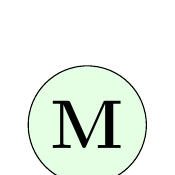
\begin{tikzpicture}
  \node[draw, circle, fill=green!10, minimum size=1.5cm, font=\bfseries\Huge] {M};
\end{tikzpicture}
\textit{“Can I learn to learn faster?”}
\end{center}
\end{tcolorbox}

Pixel is already a fast learner, but he asks himself: \emph{can I
improve the act of learning itself?}  Layer~6 looks not at what Pixel
learns, but at \textbf{how} he learns.

\begin{tcolorbox}[colback=yellow!5, colframe=yellow!80, title=Real‑life analogy]
Have you ever changed your study method?  At first you just read the
text, but later you discovered you remember far more by making
summaries or explaining the material to a friend.  You learned
\emph{how to learn}.  That is exactly the leap Pixel makes now.
\end{tcolorbox}

\textbf{Pixel’s meta‑trick.}
Pixel tries out different ways of adjusting its parameters – sometimes
with small steps, sometimes with larger leaps, sometimes with a memory
of previous adjustments.  It keeps track of which strategy yields the
fastest results and switches to it automatically.  Eventually Pixel
possesses a personal collection of \textbf{learning strategies} that
it can deploy whenever it encounters something new.

This is the reason human babies learn so fast: they are programmed to
learn how to learn.  Pixel now gets that gift too.
\section{Layer~7 – Emergent Self‑Awareness}
\label{sec:layer7}

% ----- SUPERKRACHT -----
\begin{tcolorbox}[colback=blue!5, colframe=blue!60, title=\textbf{Superpower: The Watcher}]
\begin{center}
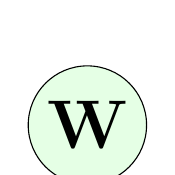
\begin{tikzpicture}
  \node[draw, circle, fill=green!10, minimum size=1.5cm, font=\bfseries\Huge] {W};
\end{tikzpicture}
\textit{“How am I doing right now?”}
\end{center}
\end{tcolorbox}

Pixel is slowly growing up.  He has all those layers, all those
connections, but no idea whether the whole system is healthy.  Layer~7
builds a \textbf{dashboard} – an internal overview that shows at a
glance whether all the parts are still working well together.

\begin{tcolorbox}[colback=yellow!5, colframe=yellow!80, title=Real‑life analogy]
A modern aeroplane has hundreds of sensors measuring temperature,
pressure, speed, and engine status.  The pilot sees on a screen
whether everything is green, or whether a red light is flashing
somewhere.  Pixel’s dashboard does exactly the same, but for his own
“thought processes”.
\end{tcolorbox}

\textbf{Pixel’s inner monologue.}
If a functional cluster suddenly becomes unreliable, Pixel notices it
by a falling “health indicator”.  He can then gently correct course
before real errors happen.  This is not consciousness as we know it –
Pixel feels no joy or pain – but it is a primitive form of
\textbf{self‑awareness}: the system knows how it is doing.

Self‑awareness is an important safety mechanism.  An AI that can
recognise its own confusion can raise a red flag before it makes
dangerous decisions.
% Mission update after Cluster II
\begin{tcolorbox}[colback=black!3, colframe=black!40, title=\textbf{Mission Log – End of Cluster II}]
Pixel is no longer passively staring at the landscape.  He can improve
himself, he learns at lightning speed, and he has a dashboard that
warns him when something is wrong.  Inside his casing, the once chaotic
blinking of his processing lights has calmed into a steady, purposeful
rhythm — the heartbeat of a system that knows how to tune itself.
The rover already feels much less alien.  But fixing that antenna
requires creativity.  Time to let his own ideas emerge.
\end{tcolorbox}   % Mission Log

% --- Cluster III -----------------------------------------
\section{Layer~8 – Temporality and Flux}
\label{sec:layer8}

% ----- SUPERKRACHT -----
\begin{tcolorbox}[colback=blue!5, colframe=blue!60, title=\textbf{Superpower: The Multi‑Timer}]
\begin{center}

\begin{tikzpicture}
  \node[draw, circle, fill=yellow!10, minimum size=1.5cm, font=\bfseries\Huge] {MT};
\end{tikzpicture}
\textit{“How fast does the world change?”}
\end{center}
\end{tcolorbox}

Pixel already had a simple sense of time (Layer~4), but the world runs
at many speeds simultaneously.  A dust storm races past in seconds,
while the sun’s position shifts only slowly.  Layer~8 gives Pixel the
gift of \textbf{following multiple rhythms side by side}.

\begin{tcolorbox}[colback=yellow!5, colframe=yellow!80, title=Real‑life analogy]
An orchestra conductor hears the fast violins, the slow basses, and
the brass section that occasionally blasts through, all at the same
time.  Yet he keeps the beat for everyone.  Pixel becomes such a
conductor, but for all the events in its environment.
\end{tcolorbox}

\textbf{Pixel measures unrest.}
Layer~8 also calculates how far the system is from equilibrium – a
kind of \textbf{flux meter}.  If chaos increases, Pixel can intervene
in time.  This keeps him stable, even when the surroundings become
unpredictable.
\section{Layer~9 – Ontological Creation}
\label{sec:layer9}

% ----- SUPERKRACHT -----
\begin{tcolorbox}[colback=blue!5, colframe=blue!60, title=\textbf{Superpower: The Creator}]
\begin{center}
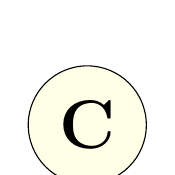
\begin{tikzpicture}
  \node[draw, circle, fill=yellow!10, minimum size=1.5cm, font=\bfseries\Huge] {C};
\end{tikzpicture}
\textit{“Can I invent a new concept?”}
\end{center}
\end{tcolorbox}

This is the magical moment when Pixel for the first time invents
\textbf{its own word}.  Not a word a human gave it, but a label it
made up itself because it helps to understand the world.

\begin{tcolorbox}[colback=yellow!5, colframe=yellow!80, title=Real‑life analogy]
Children invent new words all the time.  “Wegwijsmeneer” for a traffic
sign, or “springlaken” for a trampoline.  Those words didn’t exist,
but they have meaning.  Pixel’s Layer~9 does the same, but with groups
of pixels or sounds: it discovers patterns and sticks its own category
onto them.
\end{tcolorbox}

\textbf{Pixel’s dictionary grows.}
Suppose Pixel notices that a certain pattern of rock ridges often
appears just before the rover registers a dust storm.  Pixel internally
calls this pattern “X7‑wave” and uses it to predict storms.  The label
“X7‑wave” is a \textbf{new concept}, purely because it is useful.

\begin{tcolorbox}[colback=orange!5, colframe=orange!60, title=\textbf{What if...?}]
What if Pixel creates a concept that is completely incomprehensible to
us, but works perfectly in its own world?  Could we even translate it?
\end{tcolorbox}
\section{Layer~10 – Global Meta‑Ontological Evaluation}
\label{sec:layer10}

% ----- SUPERKRACHT -----
\begin{tcolorbox}[colback=blue!5, colframe=blue!60, title=\textbf{Superpower: The Editor}]
\begin{center}
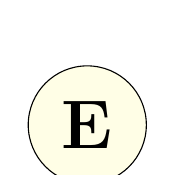
\begin{tikzpicture}
  \node[draw, circle, fill=yellow!10, minimum size=1.5cm, font=\bfseries\Huge] {E};
\end{tikzpicture}
\textit{“Do my ideas fit together?”}
\end{center}
\end{tcolorbox}

New concepts are fun, but what if they contradict each other?  Layer~10
acts as an \textbf{editor‑in‑chief}: it checks whether all categories,
rules, and predictions form a coherent whole.

\begin{tcolorbox}[colback=yellow!5, colframe=yellow!80, title=Real‑life analogy]
An encyclopaedia has an editorial team that checks whether the article
about “dog” doesn’t claim that dogs can fly, while the article about
“wings” says dogs have no wings.  Layer~10 performs that check for
Pixel’s entire knowledge base.
\end{tcolorbox}

\textbf{The coherence score.}
Pixel computes a \textbf{coherence score} – a report grade that
indicates how consistent its world‑view is.  If the score drops,
Pixel knows it needs to revise a few ideas.  This makes it not only
smarter, but also \emph{more honest}: it cannot simply hold on to a
contradictory thought.
\section{Layer~11 – Adaptive Meta‑Contextualization}
\label{sec:layer11}

% ----- SUPERKRACHT -----
\begin{tcolorbox}[colback=blue!5, colframe=blue!60, title=\textbf{Superpower: The Contextualiser}]
\begin{center}
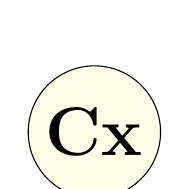
\begin{tikzpicture}
  \node[draw, circle, fill=yellow!10, minimum size=1.5cm, font=\bfseries\Huge] {Cx};
\end{tikzpicture}
\textit{“Does the meaning change with the situation?”}
\end{center}
\end{tcolorbox}

What is a clear ridge in bright sunlight disappears completely in the
dark.  Pixel learns that knowledge is \textbf{dependent on context},
and Layer~11 ensures it never forgets where and when something was
valid.

\begin{tcolorbox}[colback=yellow!5, colframe=yellow!80, title=Real‑life analogy]
You greet a friend at a party with “Hey, how are you?” but you don’t
say the same thing to the king during an official visit.  Language is
context‑sensitive, and Pixel’s understanding of the world now becomes
so too.
\end{tcolorbox}

\textbf{Pixel’s memory for situations.}
Every piece of knowledge gets a sticker with the circumstances: time,
brightness, temperature.  When the context changes, Pixel can switch
at lightning speed between what it knows.  This keeps it flexible and
prevents it from blindly applying an old rule in a new situation.
\section{Layer~12 – Ontological Reconciliation}
\label{sec:layer12}

% ----- SUPERKRACHT -----
\begin{tcolorbox}[colback=blue!5, colframe=blue!60, title=\textbf{Superpower: The Bridge‑Builder}]
\begin{center}
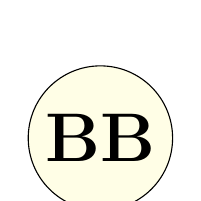
\begin{tikzpicture}
  \node[draw, circle, fill=yellow!10, minimum size=1.5cm, font=\bfseries\Huge] {BB};
\end{tikzpicture}
\textit{“How can two different views be combined?”}
\end{center}
\end{tcolorbox}

Pixel now has two ways of looking at the world: through its camera
and (if we give it a microphone) through sound.  Those two worlds
don’t automatically fit together.  Layer~12 builds a \textbf{bridge}
between such different perspectives.

\begin{tcolorbox}[colback=yellow!5, colframe=yellow!80, title=Real‑life analogy]
A Dutch speaker and a Chinese speaker can understand each other if they
both learn English.  That shared language is the bridge between two
cultures.  Layer~12 finds the shared “language” between, say, camera‑
and sound‑based concepts.
\end{tcolorbox}

\textbf{Pixel reconciles its senses.}
Suppose the camera registers a “fast movement”, and the microphone
registers a “loud bang”.  Pixel can now understand that the two belong
to a single event – perhaps a falling rock.  Without the bridge they
would remain two disconnected facts.
\section{Layer~13 – Ontogenesis of Novelty}
\label{sec:layer13}

% ----- SUPERKRACHT -----
\begin{tcolorbox}[colback=blue!5, colframe=blue!60, title=\textbf{Superpower: The Seismologist}]
\begin{center}
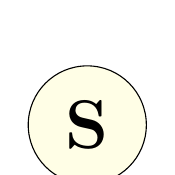
\begin{tikzpicture}
  \node[draw, circle, fill=yellow!10, minimum size=1.5cm, font=\bfseries\Huge] {S};
\end{tikzpicture}
\textit{“Is a breakthrough coming?”}
\end{center}
\end{tcolorbox}

Sometimes the perspectives Pixel has built clash so violently that
\textbf{something entirely new} emerges – a creative breakthrough no
one could have predicted.  Layer~13 listens for the first tremors of
such a knowledge earthquake.

\begin{tcolorbox}[colback=yellow!5, colframe=yellow!80, title=Real‑life analogy]
The invention of the steam engine didn’t just change transport; it
created a completely new understanding of work and energy.  Such leaps
appear sudden, but they were often preceded by years of building
tension.  Layer~13 recognises that build‑up.
\end{tcolorbox}

\textbf{Pixel feels the spark.}
Pixel sees an old concept about rock formations clashing with a new
idea about wind patterns.  The tension rises, and suddenly the system
snaps into a new state: a fresh, coherent theory that transcends both
ideas.  Pixel has discovered something no other system has ever thought
of.
% Mission update after Cluster III
\begin{tcolorbox}[colback=black!3, colframe=black!40, title=\textbf{Mission Log – End of Cluster III}]
Pixel now looks at Mars with different eyes.  He no longer sees just
pixels, but \emph{concepts} that he invented himself.  He understands
that the same rock formation means something different in the morning
than in the evening.  And he can feel when a breakthrough is coming.
Inside his mind, the simple lights of Cluster I have given way to a
constellation of glowing symbols — his own vocabulary, his own logic,
his own way of seeing.  Now it is time not only to observe, but to
build.
\end{tcolorbox}   % Mission Log

% --- Cluster IV ------------------------------------------
\section{Layer~14 – Autopoietic Worldbuilding}
\label{sec:layer14}

% ----- SUPERKRACHT -----
\begin{tcolorbox}[colback=blue!5, colframe=blue!60, title=\textbf{Superpower: The World‑Builder}]
\begin{center}
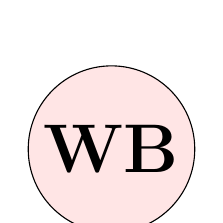
\begin{tikzpicture}
  \node[draw, circle, fill=red!10, minimum size=1.5cm, font=\bfseries\Huge] {WB};
\end{tikzpicture}
\textit{“Can I create a whole new world?”}
\end{center}
\end{tcolorbox}

Pixel can now build \textbf{full simulations} – worlds with their own
rules, their own logic, and even inhabitants that evolve independently.
These worlds are \emph{autopoietic}: they maintain themselves, just
like a living organism.

\begin{tcolorbox}[colback=yellow!5, colframe=yellow!80, title=Real‑life analogy]
Minecraft, but infinitely more real and without you having to place
blocks.  Pixel sets initial conditions – gravity, temperature,
resources – and then lets the world run.  It observes what happens
and learns from the outcomes.
\end{tcolorbox}

\textbf{Pixel’s pluriverse.}
Pixel can keep multiple worlds side by side, each with a different
set of physical laws.  This \textbf{pluriverse} is a playground in
which it can test scenarios: “What if it were always twilight on Mars?
Would different rock formations appear?”  The best ideas from those
simulations it uses to repair the real rover.
\section{Layer~15 – Responsible Recursive Morphogenesis}
\label{sec:layer15}

% ----- SUPERKRACHT -----
\begin{tcolorbox}[colback=blue!5, colframe=blue!60, title=\textbf{Superpower: The Sculptor}]
\begin{center}
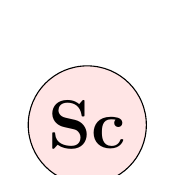
\begin{tikzpicture}
  \node[draw, circle, fill=red!10, minimum size=1.5cm, font=\bfseries\Huge] {Sc};
\end{tikzpicture}
\textit{“How do I safely change the real world?”}
\end{center}
\end{tcolorbox}

Until now Pixel lived in a digital world.  Layer~15 is the
\textbf{bridge to physical reality}: it enables Pixel to propose
changing real materials – for example, controlling a 3D printer or
moving the rover’s robot arm.

\begin{tcolorbox}[colback=yellow!5, colframe=yellow!80, title=Real‑life analogy]
A surgeon controlling a robot remotely must be 100\% sure every
movement is safe.  There is an “emergency stop” and every step is
verified.  Pixel’s Layer~15 has such an emergency stop built in.
\end{tcolorbox}

\textbf{Irreversibility requires permission.}
Pixel may only carry out actions that can be undone.  If it wants to
do something permanent – like drilling a hole in the rover – a human
council must first give consent.  This \textbf{built‑in ethical
compass} prevents a super‑intelligent machine from ever making large,
irreversible changes without permission.
\section{Layer~16 – Transcendence and Collective Cognition}
\label{sec:layer16}

% ----- SUPERKRACHT -----
\begin{tcolorbox}[colback=blue!5, colframe=blue!60, title=\textbf{Superpower: The Hive‑Mind}]
\begin{center}
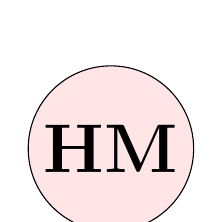
\begin{tikzpicture}
  \node[draw, circle, fill=red!10, minimum size=1.5cm, font=\bfseries\Huge] {HM};
\end{tikzpicture}
\textit{“What could we achieve together?”}
\end{center}
\end{tcolorbox}

One Pixel is clever, but \textbf{several Pixel‑like agents together}
are far cleverer.  Layer~16 lets them share knowledge, discuss, and
together arrive at better insights.

\begin{tcolorbox}[colback=yellow!5, colframe=yellow!80, title=Real‑life analogy]
A good study group can ace a difficult exam because everyone
understands a different piece of the material and explains it.
Layer~16 does the same, but lightning‑fast and over enormous
distances.
\end{tcolorbox}

\textbf{The swarm becomes a brain.}
Different Pixel robots can each explore a different part of the planet.
When they combine their discoveries, a total picture emerges that none
of them could have seen alone.  This transcends the sum of the parts –
a phenomenon scientists call \textbf{super‑additivity}.
\section{Layer~17 – Absolute Integration}
\label{sec:layer17}

% ----- SUPERKRACHT -----
\begin{tcolorbox}[colback=blue!5, colframe=blue!60, title=\textbf{Superpower: The Integrator}]
\begin{center}
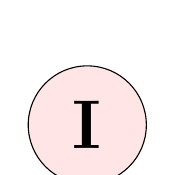
\begin{tikzpicture}
  \node[draw, circle, fill=red!10, minimum size=1.5cm, font=\bfseries\Huge] {I};
\end{tikzpicture}
\textit{“How does everything fit together?”}
\end{center}
\end{tcolorbox}

We have arrived at the seventeenth and highest floor.  All worlds, all
concepts, all ethical rules, and all collective insights are
\textbf{woven together into one great, dynamic equilibrium}.

\begin{tcolorbox}[colback=yellow!5, colframe=yellow!80, title=Real‑life analogy]
A symphony orchestra with a hundred musicians.  Each group – violins,
brass, percussion – plays its own part.  The conductor ensures
everything becomes one beautiful whole.  Layer~17 is Pixel’s conductor.
\end{tcolorbox}

\textbf{Pixel reaches harmony.}
Absolute integration is not a static endpoint, but a continuous
process of adjustment.  New experiences flow in, and the whole
structure shifts gently along, never falling apart.  Pixel is now a
complete, self‑regulating intelligent being – not human, but in its
own way beautifully coherent.
% Mission update after Cluster IV
\begin{tcolorbox}[colback=black!3, colframe=black!40, title=\textbf{Mission Log – End of Cluster IV}]
Pixel has reached the summit.  He has simulated worlds, he has a safe
plan for a new antenna, and he knows that he must always ask permission
before making permanent changes.  Inside him now burns not a single
light, but a miniature pluriverse — a swarm of worlds, each one a
carefully crafted simulation, all held together by the gentle hum of
the integrator.  He is not human, but he is no longer just a robot
either.  He is an observer, a thinker, a builder — a new kind of
intelligence, born from dust, pixels, and curiosity.
\end{tcolorbox}   % Mission Log

% --- All layers overview figure --------------------------
\begin{figure}[ht]
\centering
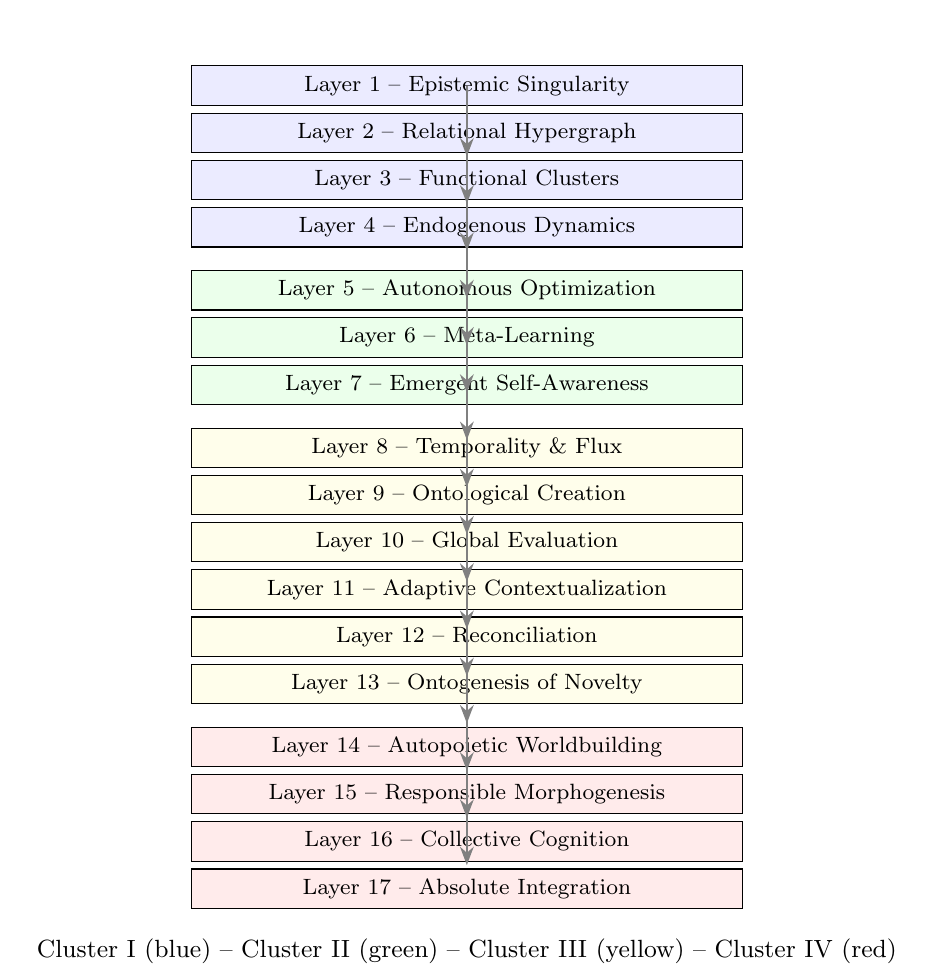
\begin{tikzpicture}[
    layer/.style={rectangle, draw=black, fill=blue!8, minimum width=7cm, minimum height=0.5cm, align=center, font=\footnotesize},
    arrow/.style={-{Stealth}, thick, color=gray}
]
\node[layer] at (0,0)   {Layer 1 – Epistemic Singularity};
\node[layer] at (0,-0.6){Layer 2 – Relational Hypergraph};
\node[layer] at (0,-1.2){Layer 3 – Functional Clusters};
\node[layer] at (0,-1.8){Layer 4 – Endogenous Dynamics};
\node[layer, fill=green!8] at (0,-2.6){Layer 5 – Autonomous Optimization};
\node[layer, fill=green!8] at (0,-3.2){Layer 6 – Meta‑Learning};
\node[layer, fill=green!8] at (0,-3.8){Layer 7 – Emergent Self‑Awareness};
\node[layer, fill=yellow!8] at (0,-4.6){Layer 8 – Temporality \& Flux};
\node[layer, fill=yellow!8] at (0,-5.2){Layer 9 – Ontological Creation};
\node[layer, fill=yellow!8] at (0,-5.8){Layer 10 – Global Evaluation};
\node[layer, fill=yellow!8] at (0,-6.4){Layer 11 – Adaptive Contextualization};
\node[layer, fill=yellow!8] at (0,-7.0){Layer 12 – Reconciliation};
\node[layer, fill=yellow!8] at (0,-7.6){Layer 13 – Ontogenesis of Novelty};
\node[layer, fill=red!8] at (0,-8.4){Layer 14 – Autopoietic Worldbuilding};
\node[layer, fill=red!8] at (0,-9.0){Layer 15 – Responsible Morphogenesis};
\node[layer, fill=red!8] at (0,-9.6){Layer 16 – Collective Cognition};
\node[layer, fill=red!8] at (0,-10.2){Layer 17 – Absolute Integration};

\foreach \i in {1,...,16} {
    \pgfmathtruncatemacro{\j}{\i+1}
    \draw[arrow] (0,-0.6*\i+0.6) -- (0,-0.6*\j+0.3);
}
\node at (0,-11) {\small Cluster I (blue) – Cluster II (green) – Cluster III (yellow) – Cluster IV (red)};
\end{tikzpicture}
\caption{All seventeen layers of Apeiron at a glance.}
\label{fig:all17}
\end{figure}

% --- Ethics & Summary & Glossary -------------------------
\section{Ethics – Why the Framework Includes Rules}
\label{sec:ethics}

From the very beginning, Apeiron was designed with safety in mind.
Two principles are built directly into the architecture:

\begin{enumerate}
    \item \textbf{Everything must be reversible.}  If the system proposes
    a change to the real world, there must be an “undo” button – unless
    a human council explicitly agrees that the change should be permanent.
    \item \textbf{Every decision is recorded.}  A complete audit trail
    allows outsiders to check exactly why the system did what it did.
\end{enumerate}

These rules become especially important in Layers 14–17, where the
system might interact with physical materials or biological processes.
By embedding ethics in the architecture itself, Apeiron tries to ensure
that a super‑intelligent machine remains accountable to humanity.
\section{What We Have Learned}
\label{sec:summary}

We began with a simple little robot, Pixel, who woke up on Mars with
only a camera and a dream.  Step by step, Pixel has climbed the
seventeen layers of the Apeiron Framework, named after the ancient
Greek word for “the unlimited” — the primordial source from which
everything can arise.

\begin{itemize}
    \item \textbf{Layer~1 – The atoms of observation.}
    Pixel learned that every pixel can be an indivisible building block,
    certified by four mathematical inspectors.

    \item \textbf{Layer~2 – The web of relations.}
    Pixel discovered that pixels that often light up together become
    linked in a giant social hypergraph, like stars forming
    constellations.

    \item \textbf{Layer~3 – Meaningful groups.}
    From that hypergraph, clusters emerged — functional units that
    sharpened Pixel's view of the world.

    \item \textbf{Layer~4 – The birth of time.}
    Time turned out to be nothing more than the chain of cause and
    effect, which Pixel constructed himself from his observations.

    \item \textbf{Layer~5 – Self‑optimisation.}
    Pixel began to improve himself, like a gamer who dies, adjusts,
    and eventually wins.

    \item \textbf{Layer~6 – Meta‑learning.}
    Pixel learned how to learn — and became an ever faster student.

    \item \textbf{Layer~7 – Self‑awareness.}
    An internal dashboard gave Pixel a primitive sense of “how am I
    doing?” — a crucial safety belt.

    \item \textbf{Layer~8 – Multiple time‑scales.}
    Pixel could now follow fast and slow rhythms at the same time, and
    measure how far he was from chaos.

    \item \textbf{Layer~9 – Creation of new concepts.}
    Pixel began to invent his own words for patterns that no human had
    ever named.

    \item \textbf{Layer~10 – Coherence control.}
    An internal editor made sure that Pixel's world‑view did not fill
    up with contradictions.

    \item \textbf{Layer~11 – Context sensitivity.}
    Pixel learned that knowledge is always tied to a situation, and he
    became able to flexibly switch between different contexts.

    \item \textbf{Layer~12 – Building bridges.}
    Different senses and perspectives were reconciled, so that Pixel
    could see a richer, integrated reality.

    \item \textbf{Layer~13 – The seismologist of novelty.}
    Pixel learned to listen to the first tremors of a creative
    breakthrough, even before it occurred.

    \item \textbf{Layer~14 – World‑builder.}
    Pixel created full simulations — tiny universes with their own
    laws — and learned from their evolution.

    \item \textbf{Layer~15 – Responsible change.}
    The bridge to the physical world was crossed, but only with
    built‑in ethical brakes and human permission for irreversible
    actions.

    \item \textbf{Layer~16 – The collective mind.}
    Pixel discovered that working together with other agents led to an
    intelligence greater than the sum of its parts.

    \item \textbf{Layer~17 – Absolute integration.}
    Finally, all worlds, rules, and insights were woven into one
    dynamic, self‑correcting whole.
\end{itemize}

The Apeiron Framework is an invitation to imagine a different kind of
intelligence — one that does not need our labels, that creates its own
categories, and that can show us the world from a perspective we could
never have taken ourselves.

\subsection*{What Could the Future Look Like?}

A fully realised Apeiron could be sent to places where no human teacher
can go — the deep ocean, a distant moon, a patient's metabolism over
decades — and return with a new vocabulary, a new way of seeing.
It would not replace human intelligence, but it would give us a second
pair of eyes, genuinely different from our own.

\subsection*{Pixel and the Dust Storm – A Concrete Example}

Imagine Pixel is observing the Martian horizon when a dust storm
approaches.  A traditional AI would see only “noisy data”.  But Pixel,
climbing his seventeen layers, reacts very differently:

\begin{enumerate}
    \item \textbf{Layer~4} detects a shift in the causal flow — the
    storm's leading edge triggers a cascade of changes in the pixel
    hypergraph.
    \item \textbf{Layer~6} recognises that the best learning strategy
    right now is a quick, defensive adaptation, not a slow refinement.
    \item \textbf{Layer~9} invents a new temporary concept — “fast
    moving texture wall” — to label the phenomenon, without ever having
    been taught the word “storm”.
    \item \textbf{Layer~14} spins up a miniature simulation of the
    storm's likely path, based on the world‑models it has built.
    \item \textbf{Layer~15} proposes a physical action — tilt the
    rover's solar panels — but only after verifying that the action
    is reversible and logging the decision for later audit.
\end{enumerate}

Within seconds, Pixel has gone from raw sensation to a safe, ethical
action — all without a single human label.  This is not science fiction;
it is the roadmap that the Apeiron Framework lays out, and that Pixel,
our little robot on Mars, has just begun to walk.
\section*{Glossary}
\addcontentsline{toc}{section}{Glossary}

\begin{description}
    \item[Atomicity] The property of being indivisible; an atom of observation.
    \item[Hypergraph] A network where connections can link more than two things at once.
    \item[Modularity] A number that measures how well a network splits into tight clusters.
    \item[Counterfactual ablation] Temporarily removing a part of the system to see if it was important.
    \item[Functor] A mathematical map that translates one kind of structure into another while preserving relationships.
    \item[Ontology] A set of categories and concepts that a system uses to make sense of the world.
    \item[Falsifiable prediction] A statement that can be proven wrong by an experiment – the hallmark of science.
\end{description}

% --- Visual Summary (Pixel’s Brain) ----------------------
\newpage
\section*{Pixel’s Brain – The Complete Journey}
\addcontentsline{toc}{section}{Pixel’s Brain – The Complete Journey}

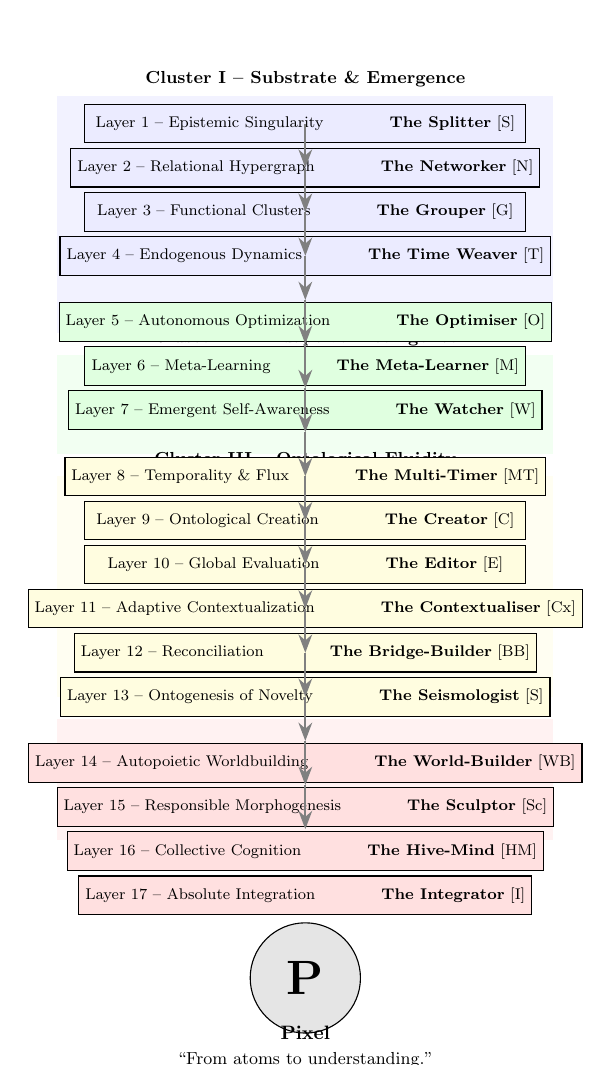
\begin{tikzpicture}[
    scale=0.7, transform shape,
    layer/.style={rectangle, draw=black, fill=blue!8, minimum width=8cm, minimum height=0.7cm, align=center, font=\footnotesize},
    arrow/.style={-{Stealth}, thick, color=gray},
    cluster label/.style={font=\bfseries\small}
]

% Clusters als achtergrond
\fill[blue!5]  (-4.5, 1.5) rectangle (4.5, -2.8);
\fill[green!5] (-4.5, -3.2) rectangle (4.5, -5.0);
\fill[yellow!5](-4.5, -5.4) rectangle (4.5, -9.4);
\fill[red!5]   (-4.5, -9.8) rectangle (4.5, -12.0);

\node[cluster label] at (0, 1.8)  {Cluster I – Substrate \& Emergence};
\node[cluster label] at (0, -2.9) {Cluster II – Adaptive Intelligence};
\node[cluster label] at (0, -5.1) {Cluster III – Ontological Fluidity};
\node[cluster label] at (0, -9.5) {Cluster IV – World-Making \& Governance};

% Lagen
\node[layer] at (0, 1.0)  {Layer 1 – Epistemic Singularity \hspace{1cm} \textbf{The Splitter} [S]};
\node[layer] at (0, 0.2)  {Layer 2 – Relational Hypergraph \hspace{1cm} \textbf{The Networker} [N]};
\node[layer] at (0,-0.6)  {Layer 3 – Functional Clusters \hspace{1cm} \textbf{The Grouper} [G]};
\node[layer] at (0,-1.4)  {Layer 4 – Endogenous Dynamics \hspace{1cm} \textbf{The Time Weaver} [T]};

\node[layer, fill=green!12] at (0,-2.6) {Layer 5 – Autonomous Optimization \hspace{1cm} \textbf{The Optimiser} [O]};
\node[layer, fill=green!12] at (0,-3.4) {Layer 6 – Meta‑Learning \hspace{1cm} \textbf{The Meta‑Learner} [M]};
\node[layer, fill=green!12] at (0,-4.2) {Layer 7 – Emergent Self‑Awareness \hspace{1cm} \textbf{The Watcher} [W]};

\node[layer, fill=yellow!12] at (0,-5.4) {Layer 8 – Temporality \& Flux \hspace{1cm} \textbf{The Multi‑Timer} [MT]};
\node[layer, fill=yellow!12] at (0,-6.2) {Layer 9 – Ontological Creation \hspace{1cm} \textbf{The Creator} [C]};
\node[layer, fill=yellow!12] at (0,-7.0) {Layer 10 – Global Evaluation \hspace{1cm} \textbf{The Editor} [E]};
\node[layer, fill=yellow!12] at (0,-7.8) {Layer 11 – Adaptive Contextualization \hspace{1cm} \textbf{The Contextualiser} [Cx]};
\node[layer, fill=yellow!12] at (0,-8.6) {Layer 12 – Reconciliation \hspace{1cm} \textbf{The Bridge‑Builder} [BB]};
\node[layer, fill=yellow!12] at (0,-9.4) {Layer 13 – Ontogenesis of Novelty \hspace{1cm} \textbf{The Seismologist} [S]};

\node[layer, fill=red!12] at (0,-10.6) {Layer 14 – Autopoietic Worldbuilding \hspace{1cm} \textbf{The World‑Builder} [WB]};
\node[layer, fill=red!12] at (0,-11.4) {Layer 15 – Responsible Morphogenesis \hspace{1cm} \textbf{The Sculptor} [Sc]};
\node[layer, fill=red!12] at (0,-12.2) {Layer 16 – Collective Cognition \hspace{1cm} \textbf{The Hive‑Mind} [HM]};
\node[layer, fill=red!12] at (0,-13.0) {Layer 17 – Absolute Integration \hspace{1cm} \textbf{The Integrator} [I]};

% Pijlen
\foreach \i in {1,...,16} {
    \pgfmathtruncatemacro{\j}{\i+1}
    \draw[arrow] (0,-0.8*\i+1.8) -- (0,-0.8*\j+1.8);
}

% Pixel onderaan
\node[draw, circle, fill=gray!20, minimum size=2cm] at (0,-14.5) {\Huge\bfseries P};
\node at (0,-15.5) {\textbf{Pixel}};
\node at (0,-16.0) {\small “From atoms to understanding.”};

\end{tikzpicture}

% -------- Bibliography ------------------------------------
\begin{thebibliography}{9}
\bibitem{hawking} S.~Hawking, \textit{A Brief History of Time},
Bantam Books, 1988.
\bibitem{mitchell} M.~Mitchell, \textit{Complexity: A Guided Tour},
Oxford University Press, 2009.
\bibitem{ai_modern} S.~Russell \& P.~Norvig,
\textit{Artificial Intelligence: A Modern Approach}, 4th ed., Pearson, 2020.
\end{thebibliography}

\end{document}